
{\Large Work in Progress - 28 january 2020}

\subsubsection{Introduction}

In parameterized convection models for planetary thermal evolution the heat transport characteristics 
of the convecting mantle are formulated in a pseudo steady state approximation. 
This is done by parameterization of the surface heatflux as a function of convective vigor, 
through the non-dimensional Nusselt number $Nu$. 
$Nu$ is usually expressed in terms of the 
Rayleigh number $Ra$ as $Nu \sim C\, Ra^\beta$, where $C$ is a constant depending on the domain geometry
(please do read section 1 of \cite{wodd09} for more information).


In this lab exercise you will investigate the characteristics of steady-state Rayleigh-Benard convection 
and determine the relation between the Nusselt and Rayleigh number experimentally, 
by means of numerical modelling. In particular you will measure the heatflow through the top surface of 
a 2D model of a convecting layer, as a function of the Rayleigh number, expressed in the temperature 
contrast across the convecting layer. 
This is done by a series of modelling experiments where the coupled equations for thermal convection are solved 
numerically using finite element methods.

The following sections contain descriptions of the numerical model and the experiments to be done. 

%........................................................
\subsubsection{Reminder of the governing model equations}

In this computerlab you will perform experiments with numerical solutions of the coupled equations describing thermal convection in an incompressible viscous fluid with infinite Prandtl number\footnote{In heat transfer problems, the Prandtl number controls the relative thickness of the momentum and thermal boundary layers. When Pr is small, it means that the heat diffuses quickly compared to the velocity (momentum).}.

In what follows, the assumption is made that geological materials can be treated as fluids (with 
special properties) within the realm of continuum fluid mechanics.
A Boussinesq approximation is applied, neglecting density variations in the equations except in the buoyancy term of the momentum conservation equation. We consider two-dimensional problems.


\begin{eqnarray}
{\vec \nabla}\cdot {\bm \sigma} + \rho(T) {\vec g} &=& {\vec 0} \label{eq_moce}\\
{\vec \nabla}\cdot {\vec \upnu} &=& 0 \label{eq_mace}\\
{\bm \sigma} &=& -p {\bm 1} + {\bm s} \label{steq}\\
{\bm s} &=& 2 \mu \dot{\bm \varepsilon} \label{stwomu}\\
\dot{\bm \varepsilon}  &=& \frac{1}{2} \left( {\vec \nabla}{\vec \upnu} 
+ ({\vec \nabla}{\vec \upnu})^T  \right) \label{epsdot} \\
\rho_0 c_p \left( \frac{\partial T}{\partial t}  + {\vec \upnu}\cdot {\vec \nabla} T\right) 
&=& {\vec \nabla}\cdot (k {\vec \nabla}T)  \label{eqhte} \\
\rho(T) &=& \rho_0 (1 - \alpha (T-T_0)) 
\end{eqnarray}

Equation (\ref{eq_moce}) is the momentum conservation equation and 
Eq. (\ref{eq_mace}) is the mass conservation equation for incompressible fluids.
One can resolve the stress tensor ${\bm \sigma}$ into its spherical part $-p{\bm 1}$ and its stress deviation ${\bm s}$ (see Eq. (\ref{steq})), where the deviatoric stress tensor is proportional to the strain rate tensor $\dot{\bm \varepsilon}$ (see Eq.(\ref{stwomu})) through the dynamic viscosity $\mu$. Finally Eq. (\ref{epsdot}) relates the strain rate tensor to the velocity field.

Equations (\ref{eq_moce}), (\ref{eq_mace}), (\ref{steq}), (\ref{stwomu}) and (\ref{epsdot}) all together lead to the following form of the Stokes equations:
\begin{eqnarray}
{\vec \nabla}\cdot [\mu ({\vec\nabla} {\vec \upnu} + {\vec \nabla} {\vec \upnu}^T ) ] 
- {\vec \nabla}p + \rho {\vec g} &=& {\vec 0} \label{mce2} \\
{\vec \nabla}\cdot {\vec \upnu} &=& 0 \label{eq_mace2}
\end{eqnarray}
Equation (\ref{mce2}) is an elliptic equation characterized by the 
fact that changes in buoyancy and constitutive relationships anywhere in the domain have an immediate influence on the entire domain.

\begin{table}
\centering
\begin{tabular}{ll}
\hline
symbol & meaning and dimension \\
\hline
\hline
${\bm g}$ & gravity acceleration vector $(m.s^{-2})$ \\
$L_x$, $L_y$ & domain size $(m)$ \\
$p$ & pressure $(Pa)$ \\
${\bm s}$ & deviatoric stress vector $(Pa)$ \\
${\bm v}=(u,v,w)$ & velocity $(m.s^{-1})$ \\
$\dot{\bm \varepsilon}$ & strain-rate tensor $(s^{-1})$ \\
$\lambda$ & penalty coefficient $(Pa.s)$ \\
$\mu$ & viscosity $(Pa.s)$ \\
$\rho,\rho_0$ & mass density $(kg.m^{-3})$ \\
${\bm \sigma}$ & stress tensor $(Pa)$ \\
$k$ & heat conductivity \\
$c_p$ & heat capacity\\
$\alpha$ & thermal expansion \\
\hline
\end{tabular}
\caption{Nomenclature \label{table_nomenc}}
\end{table}


%........................................................
\subsubsection{Numerical solution of the equations}

Introduced in the late 1950s, the finite element method (FEM) \cite{hugh,zita1,zita2,zita3} 
has emerged as one of the most powerful numerical methods so far devised. 

Quadrilateral/hexahedral $Q_1P_0$ elements (bi/tri-linear velocity, piecewise constant pressure) are used in this code.
Despite the fact that they violate the Ladyzhenskaya, Babouska and Brezzi (LBB) stability condition \cite{dohu03}, they remain a popular practical choice in mixed finite 
element approximation of incompressible materials. 

This popularity can be explained by factors such as a) local mass conservation ; b) simple and uniform data structures and algebraic problems 
with manageable sizes and small bandwidths. The latter are of paramount importance for problems 
where geometry resolution requires very fine meshes and higher order elements can quickly lead to intractable algebraic problems in three space dimensions.


The physical domain $\Omega$ is broken up into elements, and a set of finite element basis functions is defined for each element so that functional 
representations of the independent variables can be constructed.

A thorough mathematical treatment of the finite element formulation of the equations gouverning the physics of the system is beyond the scope of this 
work, and has been exposed rigorously in some key references: the reader is referred to \cite{dohu03} or \cite{gunz89} for details on the theory and implementation of viscous incompressible flows, and to \cite{lens04} for details on the theory and implementation of the heat transport equation. The FEM formulation of Eqs. (\ref{peneq}) and (\ref{eqhte}) is presented succinctly in the next section.

Even though Eqs. (\ref{peneq}) and (\ref{eqhte}) are coupled through the viscosity and density dependences on temperature and/or velocity, these equations are traditionally not solved in a coupled manner. The obtention of a new set of variables $({\bm v},p,T)$ at a given time is the product of a three-stage process:
\begin{enumerate}
\item solve for velocity field
\item recover pressure field from velocity field 
\item solve for temperature
\end{enumerate}

The size of the assembled FE matrix grows like the square of the total number of nodes, but this matrix is very sparse. Contrarily to 
optimised FE codes, no appropriate sparse storage scheme (lower triangular compressed sparse column, or CSC) is used in the code
you are going to use. This 
strongly limits the number of elements/nodes which a grid can count.

%, as this allows for a substantial reduction of memory usage.

The Galerkin finite element equation corresponding to Eq. (\ref{peneq}) is 
\[
( {\bm K}_\mu + {\bm K}_\lambda)\cdot {\bm v} = {\bm B}
\]
with
\[
{\bm K}_\mu =\int_\Omega {\bm B}^T \cdot {\bm D}_{\mu } \cdot {\bm B} \; d\Omega
\]
\[
{\bm K}_\lambda =\int_\Omega {\bm B}^T \cdot {\bm D}_{\lambda} \cdot {\bm B} \; d\Omega
\]
\[
{\bm B}=\int_\Omega {\bm N}^T \rho {\bm g} \; d\Omega
\]

\[
{\bm D}_\mu^{2D} = \mu 
\left(
\begin{array}{ccc}
2& 0& 0 \\ 
0& 2& 0 \\
0& 0& 1 
\end{array}
\right)
\quad\quad
{\bm D}_\lambda^{2D} = 
\lambda 
\left(
\begin{array}{ccc}
1 & 1& 0\\
1 & 1& 0\\
0 & 0& 1
\end{array}
\right)
\]
and where ${\bm N}$ is the vector of shape functions, and ${\bm B}$ is the matrix of spatial derivatives of the shape functions. 


The finite element equation corresponding to the heat transfer equation is
\[
{\bm M}_c\cdot \frac{\partial {\bm T}}{\partial t} + ({\bm K}_a  + {\bm K}_d)\cdot {\bm T} = {\bm F} 
\]
where
\[
{\bm M}_c=\int_\Omega {\bm N}^T \rho c_P {\bm N} \; d\Omega
\] 
\begin{equation}
{\bm K}_a=\int_\Omega ({\bm N}^\star)^T \rho c_P  {\bm v}\cdot{\bm B} \; d\Omega \label{advmat}
\end{equation}
\[
{\bm K}_d=\int_\Omega {\bm B}^T k {\bm B} \; d\Omega
\] 
\[
{\bm F}=\int_\Omega {\bm N}^T  H \; d\Omega
\]

where ${\bm T}$ is the vector of the nodal temperatures and ${\bm v}$ is the vector of nodal velocities.



%%%%%%%%%%%%%%%%%%%%%%%%%%%%%%%%%%%%%%%%%%%%%%%%%%
\subsubsection{Two-dimensional convection in a unit box}

This benchmark deals with the 2-D thermal convection of a fluid 
of infinite Prandtl number in a rectangular closed cell.
In what follows, we will focus on the case 1a, 1b, and 1c experiments as shown in \cite{blbc89}:
steady convection with constant viscosity in a square box.

The temperature is fixed to zero on top and to $\Delta T$ at the bottom, 
with reflecting symmetry at the sidewalls (i.e. $\partial_x T=0$) 
and there are no internal heat sources. 
Free-slip conditions are implemented on all boundaries. 

The Rayleigh number is given by
\begin{equation}
Ra = \frac{\alpha g_y \rho_0 \Delta T h^3 }{\kappa \nu}
=\frac{\alpha g_y \Delta T h^3 \rho^2 c_p}{k \mu}
\end{equation}

In what follows, I use the following parameter values:  
$L_x=L_y=1$,$\rho_0=c_P=k=\mu=1$, $T_0=0$, $\alpha=10^{-4}$, $g=10^{4}Ra$.
%and I run the model with $Ra=10^4,10^{5}$ and $10^6$.

The initial temperature field is given by 
\begin{equation}
T(x,y)=(1-y) - 0.01\cos(\pi x/L_x) \sin(\pi y/L_y)
\end{equation}
The perturbation in the initial temperature fields leads to 
a perturbation of the density field and sets the fluid in motion. 
Depending on the initial Rayleigh number, the system ultimately reaches a 
steady state after some time. 
%The steady-state 
%temperature fields of case 1a,b,c are shown in Fig. \ref{fig_blankenbach1}.

The root mean square of the velocity field in the whole domain is defined as 
follows:
\begin{equation}
v_{rms}= \left( \frac{1}{V_\Omega} \int_\Omega |{\bm v}|^2 \; dV \right)^{1/2} \label{eq_vrms}
\end{equation}

%was measured for a $100\times100$ grid resolution for all three cases
%and divided by the corresponding steady state values presented in \cite{blbc89}. 
%Results are shown in Fig. \ref{fig_blankenbach2} and one 
%sees that there is a very good agreement as all three curves ultimately 
%converge to the expected value 1.

The Nusselt number (i.e. the mean surface temperature gradient over mean bottom temperature)
is computed as follows \cite{blbc89}:
\begin{equation}
Nu = L_y \frac{\int \frac{\partial T}{\partial y}(y=L_y) dx  }{\int T(y=0) dx}
\label{eqNu}
\end{equation}
Note that in our case the denominator is equal to 1 since $L_x=1$ and the temperature at the 
bottom is prescribed to be 1.

%The case 1a results are shown in Fig. \ref{fig_blankenbach3} for three grid resolutions.  
%We see that the Nusselt number converges towards the expected value and that with 
%increasing resolution the error decreases. 
%The relative error on the Nusselt number has been measured for 
%various grid resolutions with $Ra=10^4$ and %is shown in Fig. (\ref{fig_blankenbach4}).
%was found to decrease quadratically with the element size.

Finally, the steady state root mean square velocity and Nusselt number measurements
are indicated in Table \ref{tab_bl} alongside those of \cite{blbc89} and \cite{tack94}.
(Note that this benchmark was also carried out and published in 
other publications \cite{trha98,albe00,gery10,dawk11,lezh11} but since they did not provide  a complete set 
of measurement values, they are not included in the table.)

%The results obtained with {\sc elefant} compare favourably to those 
%initially published by \cite{blbc89} and fall within $1\%$ of the expected values. 



%Finally, the steady state root mean square velocity and Nusselt number measurements
%of Blankenbach et al, and those obtained with Aspect are indicated in Table (\ref{tab_bl}).
%(Note that this benchmark was also carried out an published in 
%other publications \cite{trha98, gery10, dawk11} but since they did not provide  a complete set 
%of measurement values, they were not included in the table.)

\begin{table}
\centering
\begin{tabular}{llcc}
\hline
          &           & Blankenbach et al & Tackley \cite{tack94}    \\
\hline
\hline
$Ra=10^4$ & $V_{rms}$ &  $42.864947  \pm 0.000020$ & 42.775 \\
          & $Nu$      &  $4.884409   \pm 0.000010$ & 4.878  \\
$Ra=10^5$ & $V_{rms}$ &  $193.21454  \pm 0.00010 $ & 193.11 \\
          & $Nu$      &  $10.534095  \pm 0.000010$ & 10.531 \\
$Ra=10^6$ & $V_{rms}$ &  $833.98977  \pm 0.00020 $ & 833.55 \\
          & $Nu$      &  $21.972465  \pm 0.000020$ & 21.998 \\
\hline
\end{tabular} 
\caption{Steady state Nusselt number $Nu$ and $V_{rms}$ measurements as reported in the literature.  \label{tab_bl}}
\end{table}







%\begin{figure}
%\centering
%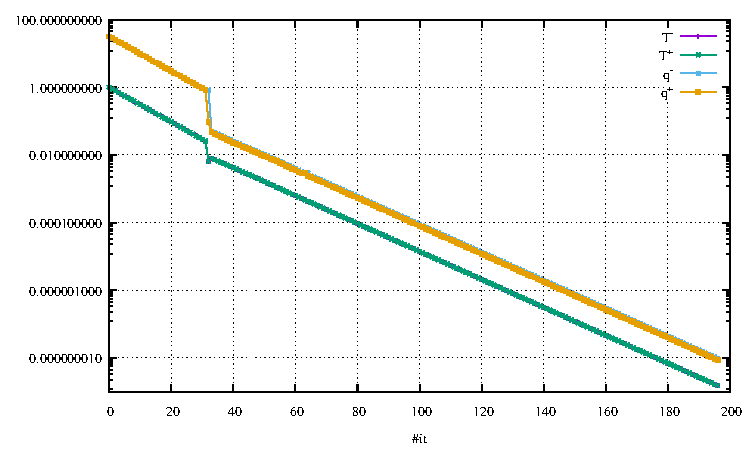
\includegraphics[width=8cm]{blankenbach/convergence.pdf}
%\caption{Steady state Nusselt number as a function of the element size. \label{fig_blankenbach4}}
%\end{figure}

%%%%%%%%%%%%%%%%%%%%%%%%%%%%%%%%%%%%%%%
\subsubsection{Experiments}

The code is to be downloaded there {\tt http://cedricthieulot.net/mantledynamics.html} . 


\begin{itemize}
\item Determine the Nusselt number at steady state for a range of Rayleigh numbers, 
starting from a subcritical value. 
Collect the Rayleigh and Nusselt numbers in a 2-column ascii file and produce a plot of Nu against Ra using double logarithmic axes with
gnuplot.
\item Determine the logarithmic slope or powerlaw index $\beta$ defined in the introduction.

\item produce such a curve for various grid resolutions. How can you explain the differences in the results ? Produce a plot 
of $Nu$ as a function of the grid spacing. Discuss.

\item Look at how the $v_{rms}$ values at steady state depend on $Ra$. 

\item For three contrasting $Ra$ values, plot the temperature profiles (data to be found in {\tt Tavrg.dat}) on a single plot and discuss the obtained figure.

\item Set the number of points in the horizontal directions to 25. Choose $Ra=10^5$ and progressively increase the number 
of points in the vertical direction. Report on the variation of the $Nu$ number at steady state as a function of the vertical
resolution.

\item Estimate the value of the critical Rayleigh number from your Nusselt number plot and investigate the 
difference with the value found in Rayleigh's linear stability analysis for a layer of depth $h$ and infinite horizontal extent, 
$Ra_C = (27/4)  \pi^4$.

\item The modelling program produces data files containing ‘snapshots’ of the resulting numerical solution 
of the temperature and velocity fields in a suitable format ({\tt .vtu}) for visualization with graphics program {\sl paraview}. 
Produce colorplots with paraview of the temperature field, for three contrasting Rayleigh number cases, and discuss them.

\item Explore the effect of the aspect ratio of the domain on $Ra_c$ and the slope $\beta$.

\item Change the initial temperature profile to something more random, repeat some of these experiments. What can you conclude ?

\end{itemize}



\newpage

\begin{itemize}
\item Rayleigh number for convection driven by a hot base (constant temperature) and a cold surface:	
\[
Ra 
= \frac{\alpha g_y \rho_0 h^3 }{\kappa \eta} \cdot (T_{bot}-T_{top})
=\frac{\alpha g_y h^3 \rho^2 c_p}{k \eta}\cdot (T_{bot}-T_{top})
\]
\item Rayleigh number	for convection driven by a hot base (constant heat flow $Q_{bot}$) and a cold surface:	
\[
Ra = \frac{\alpha g_y \rho_0 h^3 }{\kappa \eta} \cdot \frac{Q_{bot} h }{k}
\]
\item Rayleigh  number for  convection  driven  by  internal  heating
\[
Ra = \frac{\alpha g_y \rho_0 h^3 }{\kappa \eta} \cdot \frac{H h^2 }{k}
\]
where $H$ is the radiogenic heat production per cubic meter.
\item Rayleigh number for convection driven by both basal heat flow and internal heating
\[
Ra = \frac{\alpha g_y \rho_0 h^3 }{\kappa \eta} \cdot \frac{Q_{bot} h + H h^2 }{k}
\]
Note that the second term in the Rayleigh numbers describes the heating mode.
\end{itemize}


